\subsection{Opstelling}\label{sec:opstelling}
In de opstelling om de testen uit te voeren is er een server gebruikt waar alle clients zich op aansluiten aan de hand van een socket protocol. Met een knop op de pagina worden alle klokken gesynchroniseerd met de server door het tijdsverschil en de vertraging (ping) tussen de laatste twee te berekenen.
Het tijdsverschil wordt namelijk 10 keer herberekend om daaruit mogelijke verbindingsfluctuaties uit te kunnen filteren (meer hierover in sectie \ref{sec:testen}).

\begin{figure}[h]
\centering
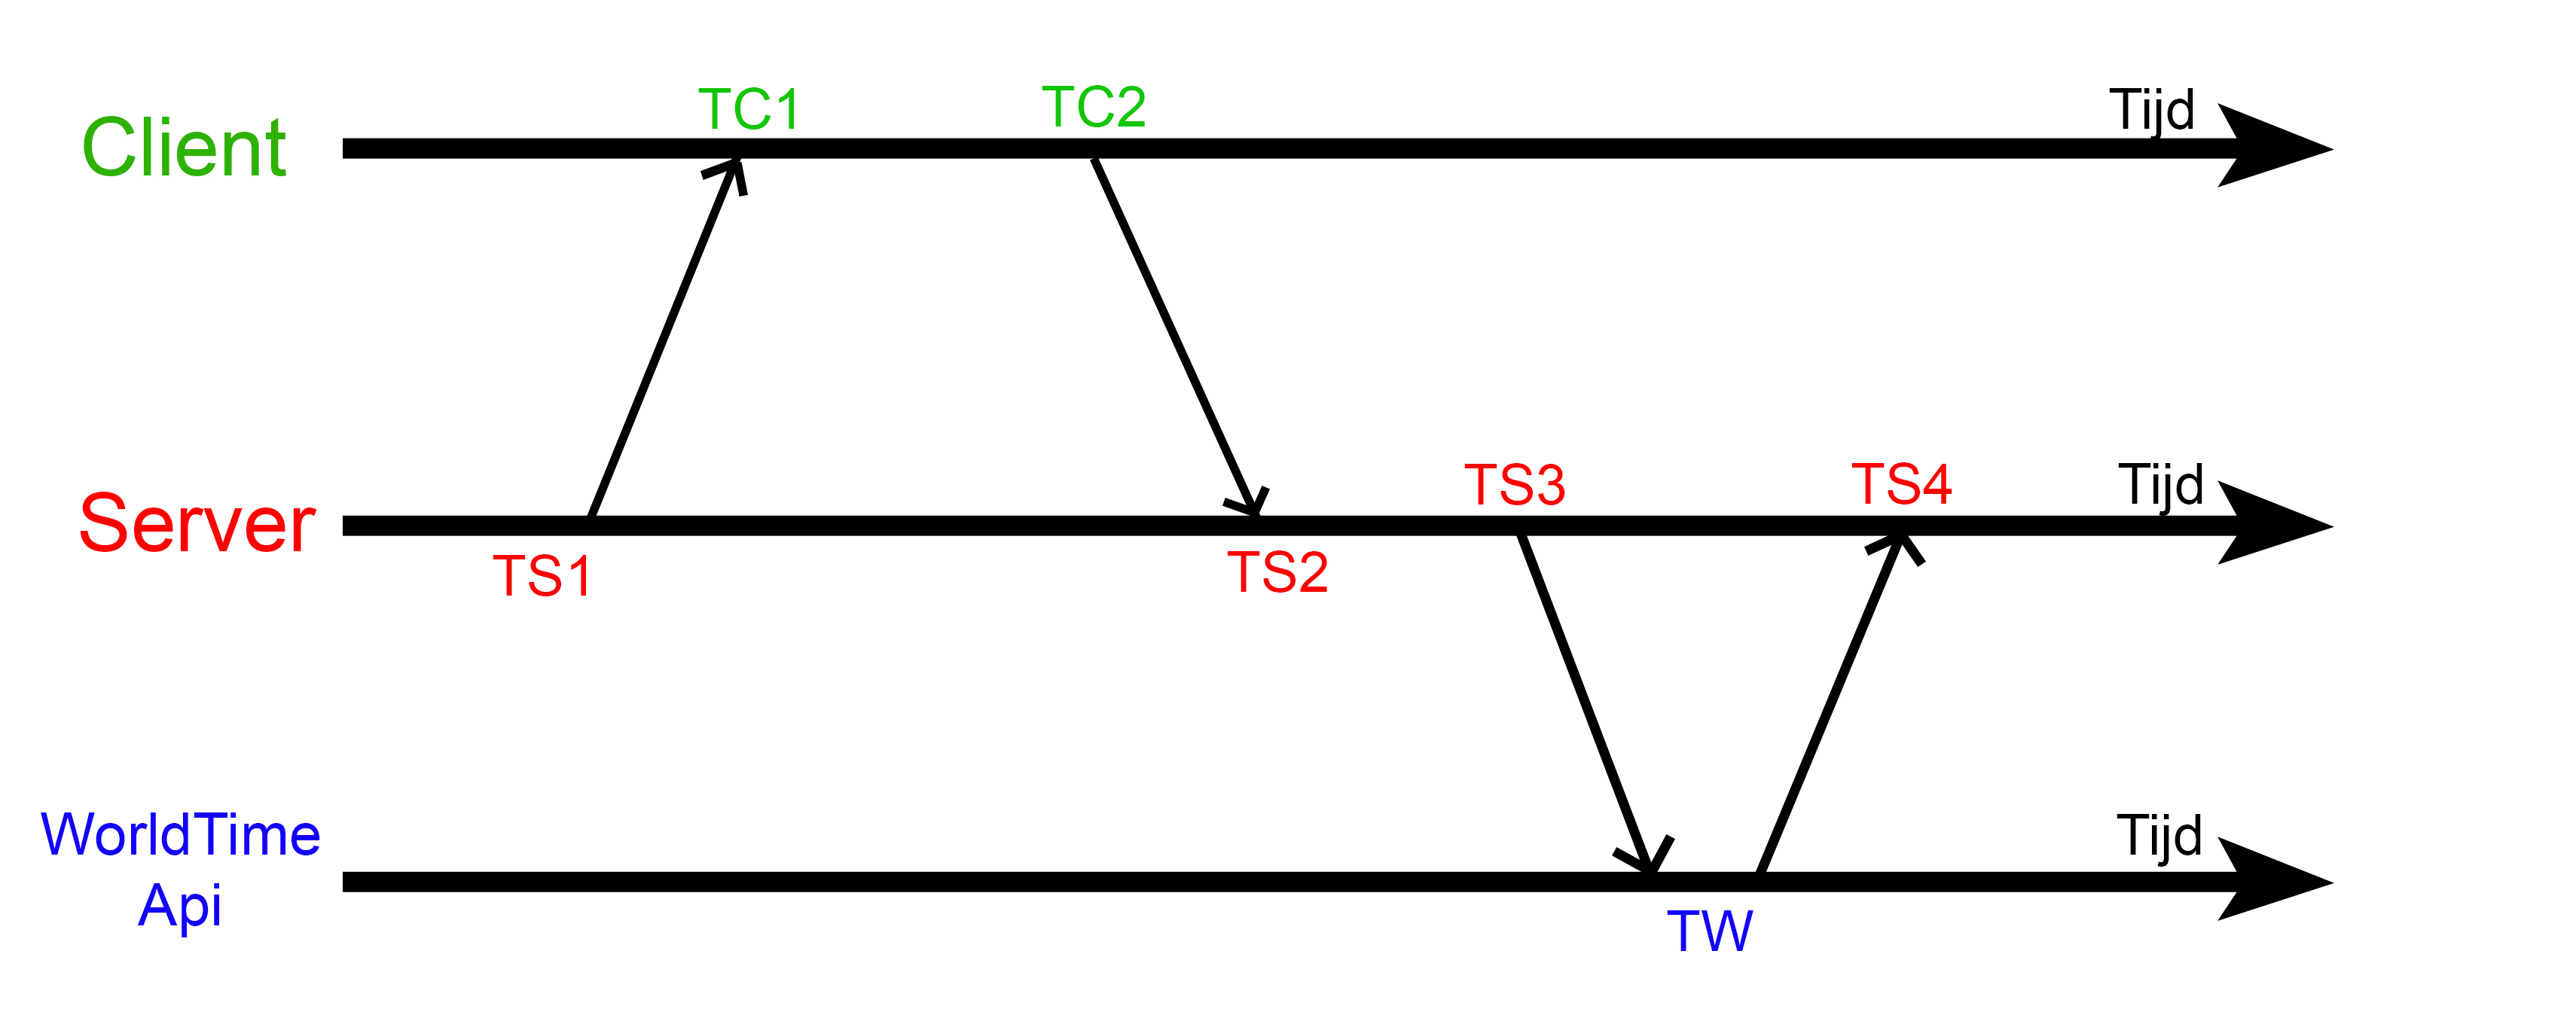
\includegraphics[scale=0.4]{img/server-client-sync.jpg}
\caption{NTP Protocol} \label{serv-client}
\end{figure}

Voor de synchronisatie is het NTP protocol geïmplementeerd. \cite{NTP:1}
Het schema over het NTP protocol is te vinden in figuur \ref{serv-client}. TSx en TCx zijn de tijden (in milliseconden) gemeten door de server en respectievelijk de client.
Het tijdsverschil wordt gemeten door.
\newline
\[ timeDiff = \frac{(TC1 - TS1) + (TS2 - TC2)}{2}  \]

De vertraging voor de server om een bericht te verzenden en terug te ontvangen is:

\[ ping  = (TS2 - TS2) - (TC2 - TC1) \]


Hiermee is het makkelijk de servertijd te berekenen door de vergelijking:

\[ timeServer = timeClient - timeDiff \]

Om vervolgens de tijdsverschil tussen de server- en de wereldtijd te berekenen is er gebruikt gemaakt van een externe API, worldtimeapi.org. Het tijdsverschil is als volgt berekend:

\[ serverWorldOffset = (TW - TS4) + \frac{TS4 - TS3}{2} \]

Uiteindelijk is de volgende informatie opgeslagen:

\begin{itemize}
  \item lijst van ping tussen client en server
  \item standaardafwijking van de ping
  \item tijdsverschil tussen client en server tijd
  \item tijdsverschil server en wereldtijd
  \item tijdsverschil client en wereldtijd
\end{itemize}






\subsection{UDP vs TCP}

UDP heeft in tegenstelling tot TCP geen gevestigde verbinding nodig tussen bijvoorbeeld server en client. TCP zal garanderen dat data correct aankomt door middel van foutopsporing en zal ook in de goede volgorde binnenstromen. Om geen pakketten te verliezen zal TCP deze in een {\it receive buffer} steken en zal de applicatie de ontvangen data pas lezen als ze er klaar voor is. Tegenover UDP waar de data continu zal binnenstromen, ontvangen of niet. Deze zal ook niet aan foutopsporing doen en de juiste volgorde niet garanderen. Het is duidelijk dat UDP veel sneller is doordat deze minder stappen en controle bevat. Nochtans is het niet mogelijk het UDP protocol te gebruiken omdat browsers deze functionaliteit niet bevatten. Daarom is er nu gebruik gemaakt van Socket.io dat met het TCP protocol werkt.

\subsection{Drift en skew}

Drift zal ervoor zorgen dat een klok niet meer synchroon met zijn oorspronkelijke referentie loopt. Windows lost dit op met een wekelijkse resync (het tijdsverschil zal dus op een sawtooth diagram lijken) terwijl Mac OSX rekening zal houden met de klok skew en andere hardware invloeden om zo beter synchroon te blijven.
Klok skew is het verschil van tijd van een kloksignaal tussen 2 componenten binnen een systeem(zie figuur \ref{skew1} \cite{skew}).

Het tijdsverschil van een windowscomputer en een atoomklok is gedurende 25 minuten gemeten (zie figuur \ref{drift}). De trendlijn is door de grafiek getrokken en het is duidelijk dat er geen effect ervan te zien is. Over langere tijdsperiode zal de drift groter worden, maar voor de animatie zal dit verwaarloosbaar zijn aangezien het onwaarschijnlijk is dat iemand dagenlang deze zal laten afspelen.

\begin{figure}[H]
\centering
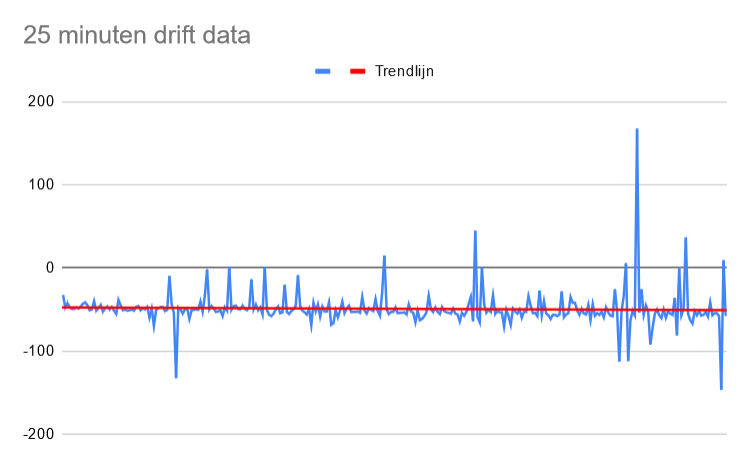
\includegraphics[scale=0.3]{img/drift.png}
\caption{Drift} \label{drift}
\end{figure}

\begin{figure}[H]
\centering
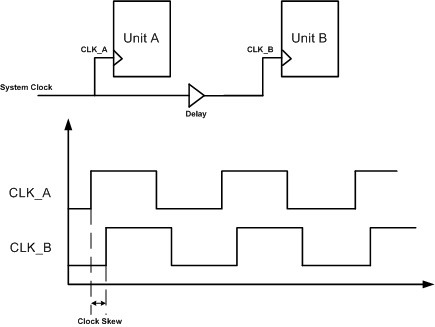
\includegraphics[scale=0.7]{img/skew.jpg}
\caption{Skew} \label{skew1}
\end{figure}


Klok skew kan problemen geven voor correct timing, en zoals eerder vermeld zal OSX dit tegen gaan via software. We zullen niet dieper gaan over de problemen van skew en OSX. 


\subsection{Analyse van de data}
\label{analyse}
Als premisse is er gesteld dat de aangesloten clients gesynchroniseerd zouden zijn met de wereldklok, gebruikmakend van het interne synchronisatiesysteem op elk toestel. Het is duidelijk in figuur \ref{fig:mediaan} dat er op elk soort systeem een afwijking gemeten wordt tegenover de referentieklok. Bij sommige operating systems al een groter verschil dan de andere, maar de reden waarom is niet altijd te verklaren of vrijgegeven en zullen hier dus niet verder op in gaan. Om dit te testen is er een poging gedaan om het verschil tussen device-klok en server-klok te vergelijken door de ping mee in rekening te brengen. De drift van beide klokken gaan over deze tijdsspan minimaal zijn en gaan geen invloed hebben op deze verschillen. Bij de testen werd ook de gemiddelde ping en standaardafwijking van de ping per test opgeslagen. Uit deze waarden valt af te leiden dat er bij grote ping fluctuaties ook een grote standaardafwijking mee gepaard ging en wijst naar inconsistenties binnen het netwerk van ofwel de client ofwel de belasting op de server en is er bijgevolg meer kans op een grotere fout binnen de vergelijking van de klokken.

\begin{figure}[H]
	\centering
	\begin{subfigure}{.5\textwidth}
		\centering
		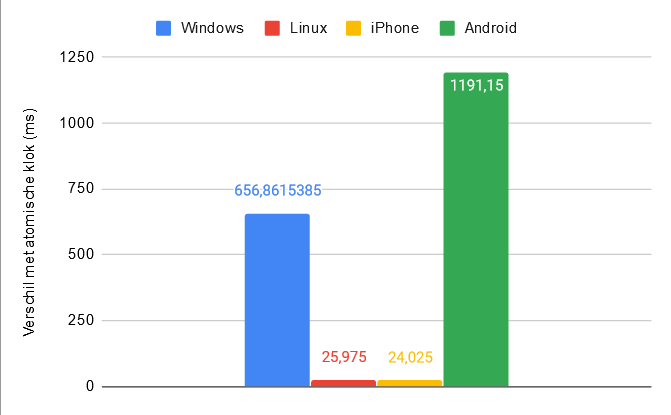
\includegraphics[width=.95\linewidth]{img/mediaan.png}
		\caption{Mediaan van tijdsverschil van elk device.}
		\label{fig:mediaan}
	\end{subfigure}%
	\begin{subfigure}{.5\textwidth}
		\centering
		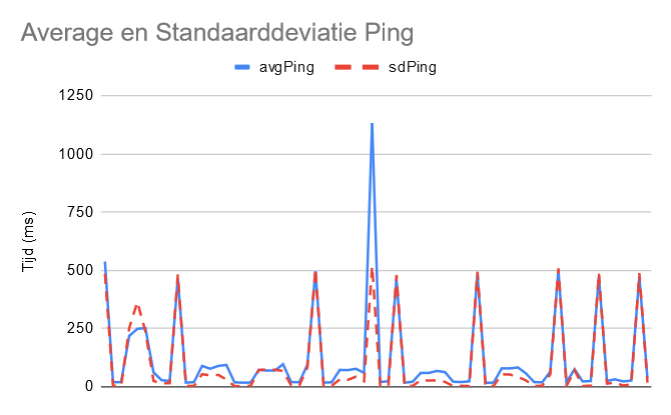
\includegraphics[width=.95\linewidth]{img/ping_results.png}
		\caption{Gemiddelde en standaardafwijking van de ping met de server. }
		\label{fig:avgPing}
	\end{subfigure}
	\caption{Resultaten van de testen}
	\label{fig:results}
\end{figure}

In figuur \ref{fig:avgPing} is het duidelijk zichtbaar dat er een pieken zijn met hoge standaardafwijkingen. Dit wilt zeggen dat er heel grote fluctuaties zijn in de ping tijdens het synchronisatieproces met 10 metingen. Hiermee zal de gesynchroniseerde tijd een afwijking hebben met de werkelijke tijd tot +-($maxPing - minPing$) milliseconden.




















